\section{Introduction}
\label{sec:intro}

Evolving graphs can be used to represent a wide range of phenomena,
including the Web, social networks, communication and transportation
networks, interaction networks, metabolism pathways, and many others.
Researchers study graph evolution rate and mechanisms, impact of
specific events on further evolution, spatial and spatio-temporal
patterns, and how graph properties change over time.  \eat{We need a
  graph model that can support these types of analyses.}

\begin{figure}[b]
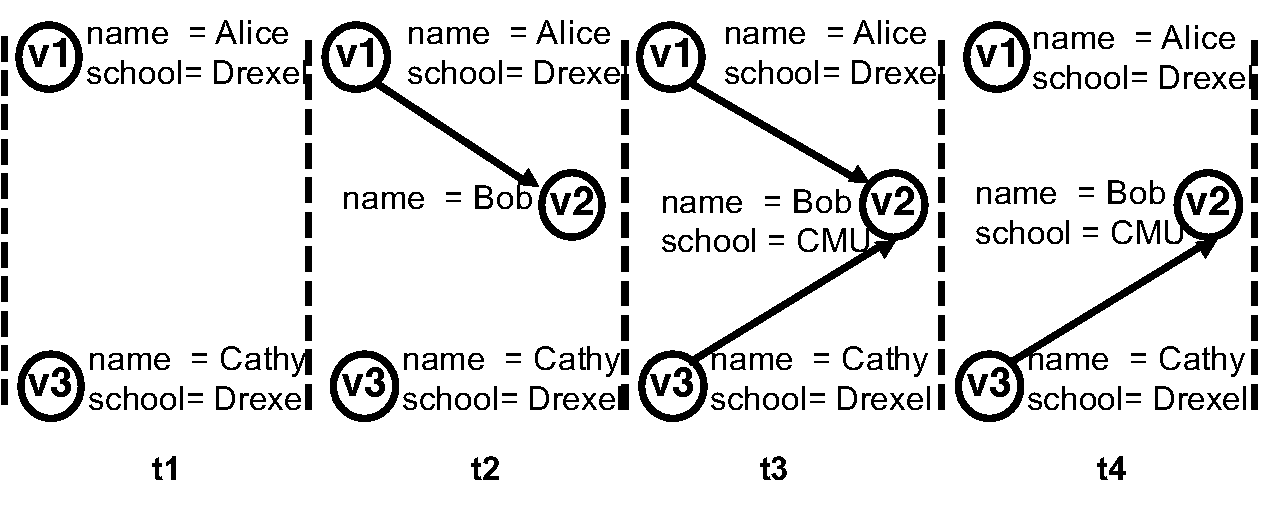
\includegraphics[width=3.4in]{figs/T1_graphs.pdf}
\vspace{-0.5cm}
\caption{Example social network as a snapshot sequence.}
%\vspace{-0.4cm}
\label{fig:snapshots}
\end{figure}

The dominant logical model for evolving graphs over the past 20 years
has been a sequence of static graphs, termed {\em snapshots}.  This
model introduces a semantic ambiguity that has been well studied in
the temporal relational databases literature~\cite{Bohlen1998}: if an
entity, i.e., node or edge, with the same attributes exists in two
consecutive snapshots, does it represent the same thing or a different
one?  What does it mean for an entity to change?
Figure~\ref{fig:snapshots} shows an example evolving social network
over four time points.  The nodes in this network are people, while
the edges are the interactions between them such as likes and
conversations.  In our example, did Alice and Bob have two
conversations over time period $[t1, t4)$ or one long one?  Did Alice
  undergo any changes during this time?  What is the rate of change of
  this evolving graph?  Which user was the most active in this network
  over its lifetime?  We cannot answer these questions without
  additional information based on this model.  Suppose Alice had a
  temporary position at Drexel at time $t1$ and was able to get a
  permanent one at time $t2$.  Alice and Bob had two interactions,
  while Cathy and Bob had one longer one.  The model cannot
  distinguish between the two cases.

This kind of semantic ambiguity affects several graph operations, most
notably aggregation and retrieval of change history, and, as a result,
local (confined to specific entity or subset of entities) and global
(whole-graph) temporal queries that are useful for evolving graphs
analysis.

\begin{figure}[t]
\vspace{-1cm}
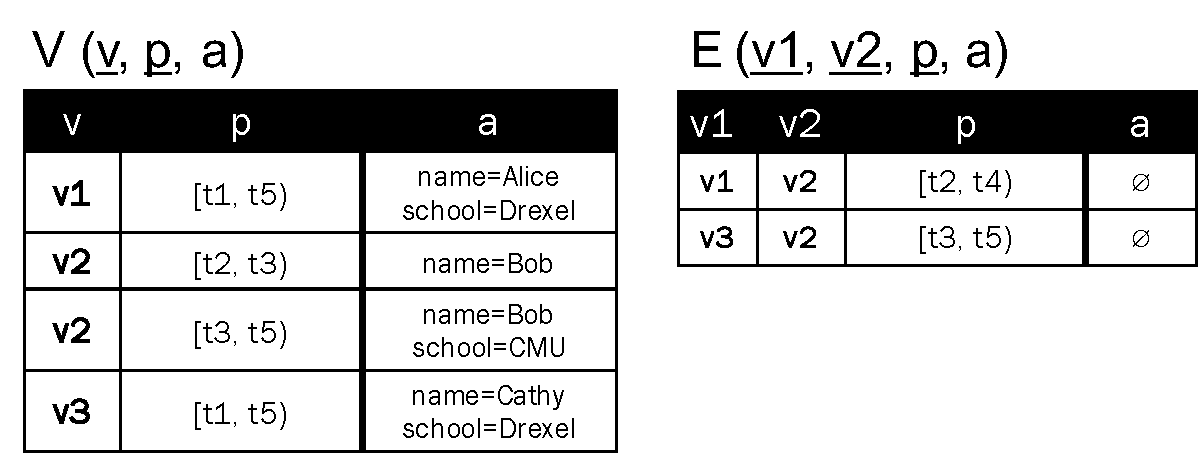
\includegraphics[width=3in]{figs/T1_relations.pdf}
\vspace{-0.2cm}
\caption{Coalesced temporal relations representing evolving graph in Figure~\ref{fig:snapshots}.}
\vspace{-0.5cm}
\label{fig:coalesced}
\end{figure}

A snapshot sequence is a graph-specific adaptation of the point-based
time model~\cite{Toman2009}.  In point-based models each entity is
time-stamped with its validity time.  For practical considerations
intervals are often used as syntactic abbreviations for sets of
points, as the pure point-based model is obviously inefficient.  To
use intervals in a time-stamped model, we coalesce, i.e., merge
value-equivalent tuples over overlapping and adjacent time
points~\cite{Bohlen09}.  In Figure~\ref{fig:coalesced} the result of
coalesced representation from Figure~\ref{fig:snapshots} is shown,
using one temporal relation for nodes and another for edges.
Attributes are represented as a set of key-value pairs based on the
property graph model~\cite{Angles2008}.

However, the use of intervals to represent a sequence of equivalent
time-adjacent snapshots is not semantically equivalent to a model with
sequenced semantics, where entities are time-stamped with intervals
that have meaning.  Note that Alice shows no changes during the whole
time interval, with a single tuple over $[t1, t4)$.  Similarly, two
  interactions between Alice and Bob are coalesced into one.  A
  work-around to avoid coalescing tuples that should not be coalesced
  is to add attributes to entities in order to distinguish between
  changes and non-changes.  We can add position title to Alice node
  and conversation id to each edge.  This solution is ad-hoc rather
  than general and does not hold up over time, as discussed
  in~\cite{Bohlen1998}.

\eat{With sequenced semantics Alice is represented with two tuples,
  one for each interval corresponding to a separate position.}

We contend that a snapshot sequence model of evolving graphs is
insufficient for representation of a wide range of networks.  We gave
an example above, but in general any network where consecutive tuples
may represent different entities while being value-equivalent is
affected.  Interaction networks, such as message exchange graphs,
epidemic transmission networks, network topologies, and any graphs
with events as edges are cases where this issue is more likely to
appear (the graphic example above is of an interaction network).
Besides the semantic ambiguity problem, many queries cannot be
formulated over the snapshot sequence model.  In particular, any query
with a temporal predicate, e.g., compute a subgraph containing only
vertices that persist for at least a year, cannot be formulated over
the snapshot sequence because semantically the query is computed
independently in each snapshot.

We propose to use the interval model with sequenced semantics to
represent evolving graphs.  In Section~\ref{sec:related} we briefly
survey existing models and summarize relevant work in temporal
databases.  We then propose a new model in Section~\ref{sec:model} and
discuss its properties.  In Section~\ref{sec:consider} we discuss the
particular challenges of efficient computation over evolving graphs in
a distributed environment and conclude with future research directions
in Section~\ref{sec:conc}.
